\section{Results}\label{sec:results}
According to equation \eqref{eq:farfield} and the specified approximations the interference pattern can be calculated using
the 2 dimensional fourier transform of the shape of the slit, Taking the inverse fourier transform of the pattern should result
In the square of the shape of the slit (since when calculating the intensity the square of $U$ was taken)
as can be shown by Fig.\ref{fig:expansion theory measurements}
\begin{figure}[H]
    \centering
    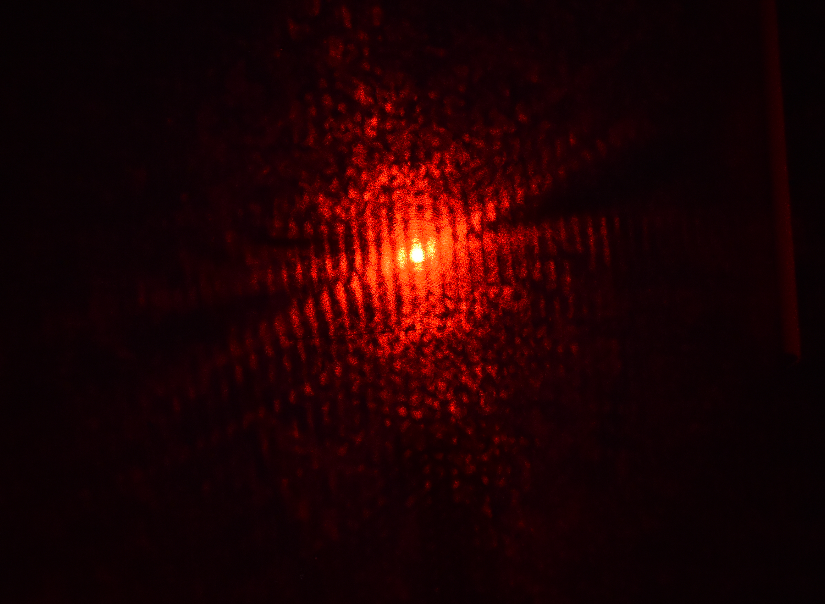
\includegraphics[width=0.9\columnwidth]{figures/expantion meshured interferemce.png}
    \caption{interference pattern measured as a result of diffraction with a helix}
    \label{fig:expansion measured interference pattern}
\end{figure}
\begin{figure}[H]
    \centering
    \begin{subfigure}{0.48\columnwidth}
        \centering
        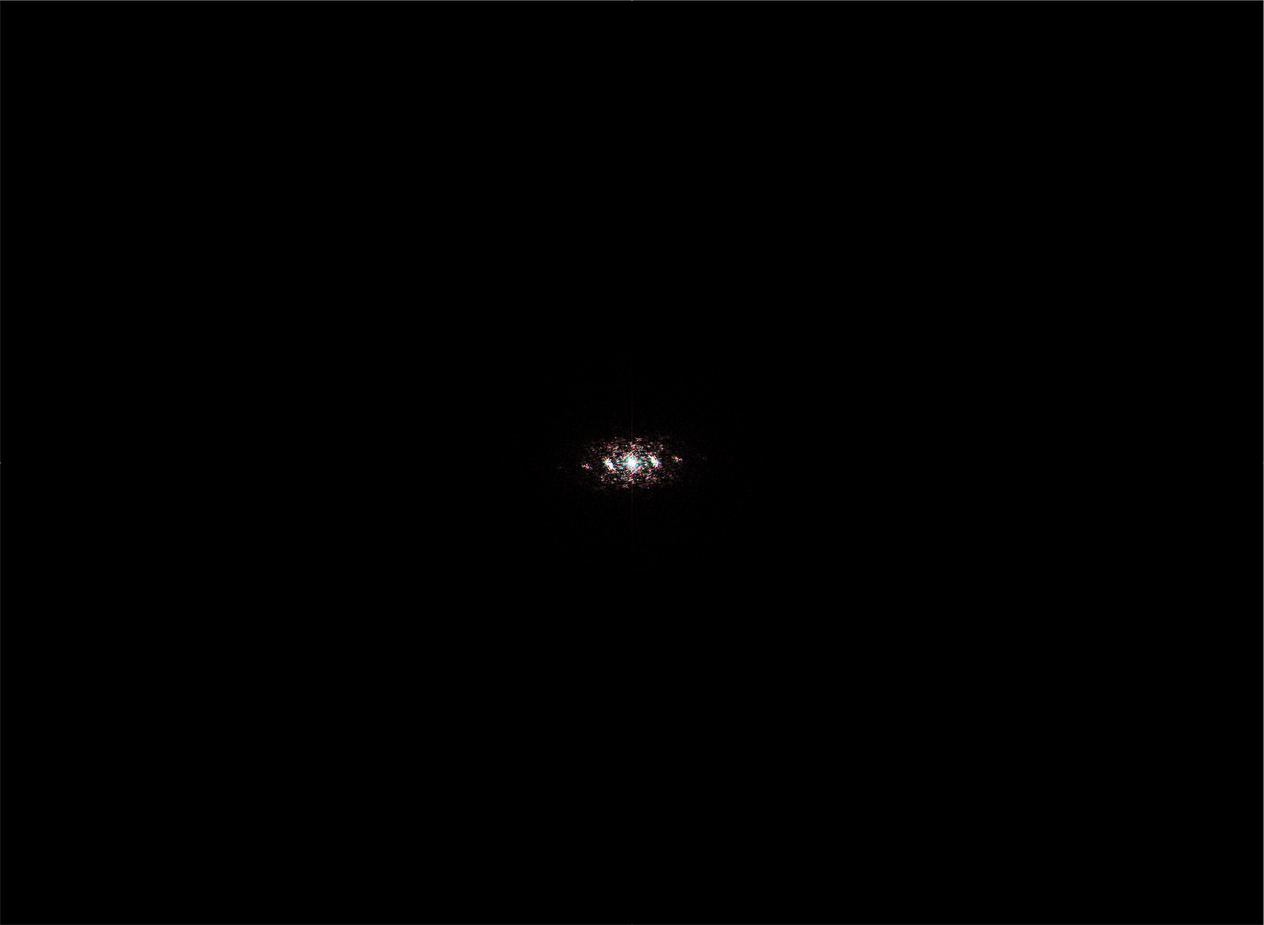
\includegraphics[width=0.9\columnwidth]{figures/expantion fourie transform.png}
        \caption{inverse discrete fourie transform calculated from the interference pattern at of the helix }
        \label{fig:expansion inverse fourie transform measured}
    \end{subfigure}\hfill
    \begin{subfigure}{0.48\columnwidth}
        \centering
        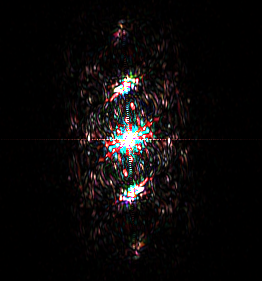
\includegraphics[width=\columnwidth]{figures/expantion fourie transform magnified.png} % second figure itself
        \caption{magnification of\ref{fig:expansion inverse fourie transform measured}}
        \label{fig:expansion fourie transform magnified}
    \end{subfigure}

    \label{fig:expansion theory measurements}
\end{figure}

While far from identical, the two images have some similarities, the bright section in the middle of the "squared helix" and the darker rings around it.
To be able to further analyse the diffraction pattern of a helix let us deconstruct it into segments.
Slit patterns can be thought of as an approximation of one-dimensional sections of a helix, they also have a well-known solution which we have confirmed by measuring the diffractions from those slit patterns.

\begin{figure}[H]
    \centering
    \begin{subfigure}{0.48\columnwidth}
        \centering
        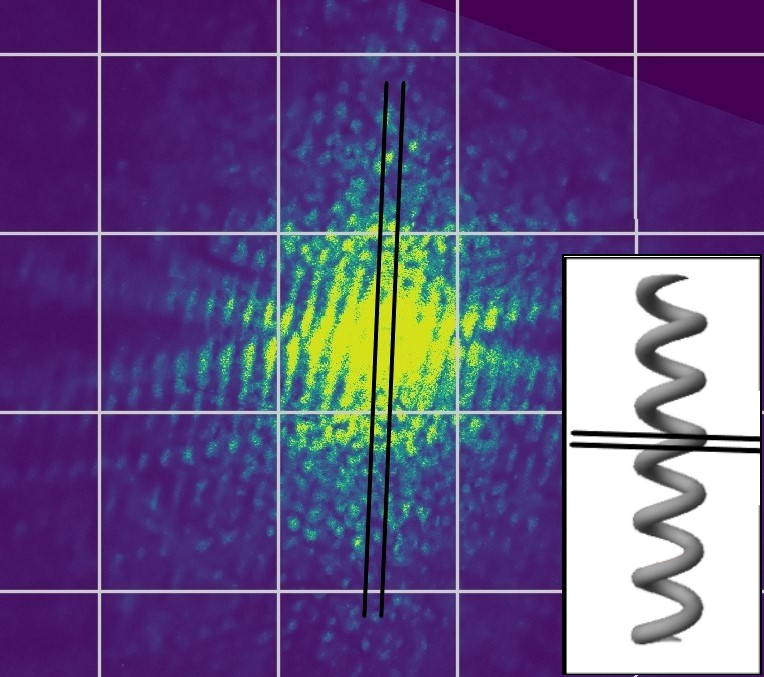
\includegraphics[width=\columnwidth]{figures/HelixSection2.png} % second figure itself
        \caption{Single slit section}
        \label{fig:HelixSection1}
    \end{subfigure}
    \begin{subfigure}{0.48\columnwidth}
        \centering
        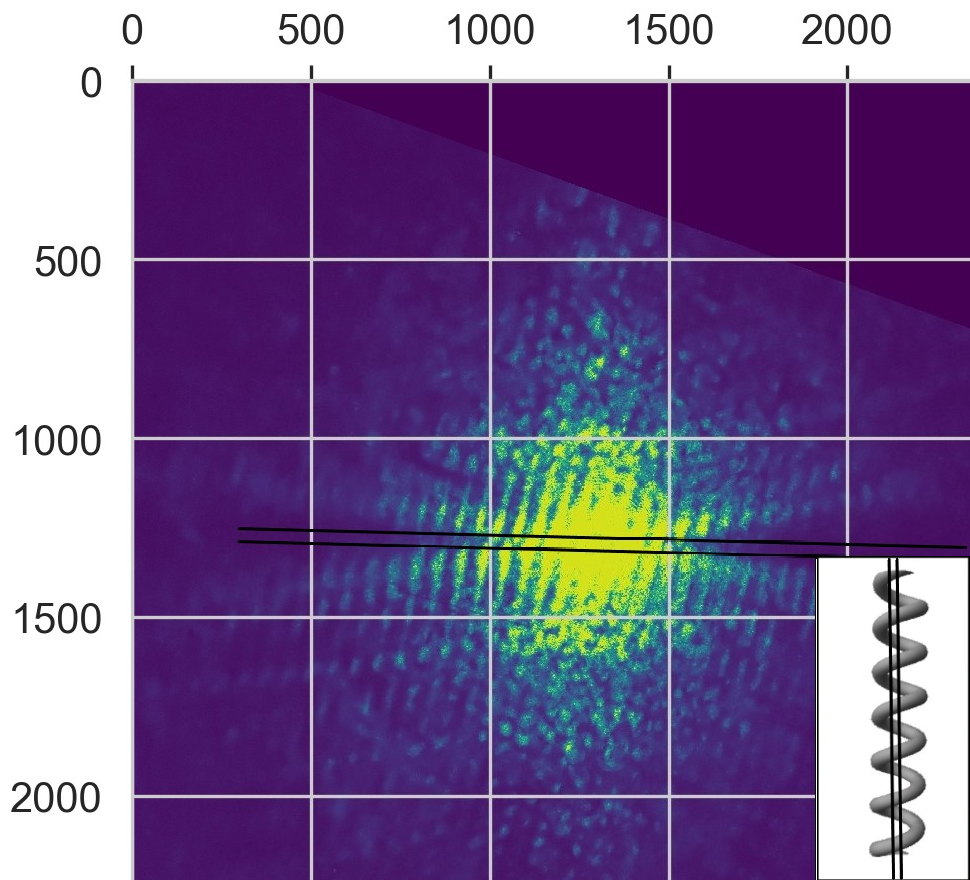
\includegraphics[width=\columnwidth]{figures/HelixSection1.png}
        \caption{N-slits section}
        \label{fig:HelixSection2}
    \end{subfigure}
    \begin{subfigure}{0.46\columnwidth}
        \centering
        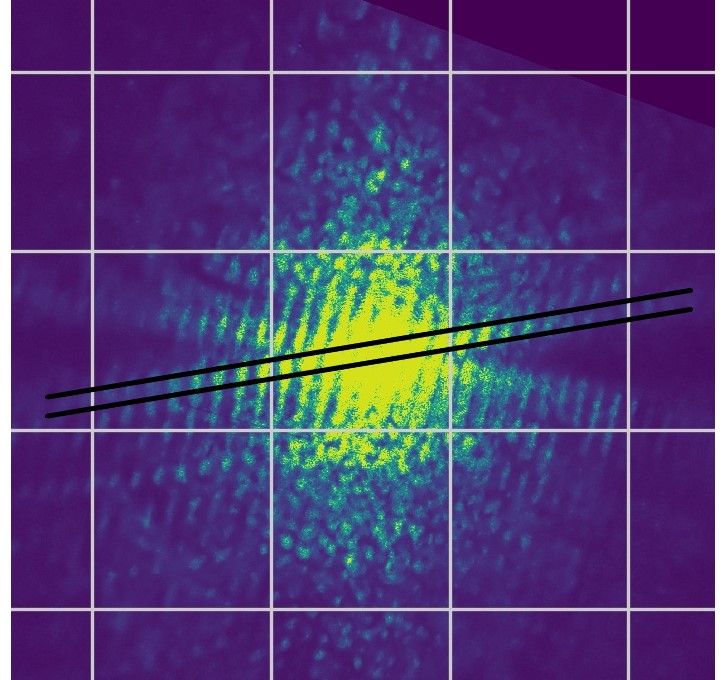
\includegraphics[width=\columnwidth]{figures/HelixSection4.jpg} % second figure itself
        \caption{"X" section 1}
        \label{fig:HelixSection3}
    \end{subfigure}
    \begin{subfigure}{0.48\columnwidth}
        \centering
        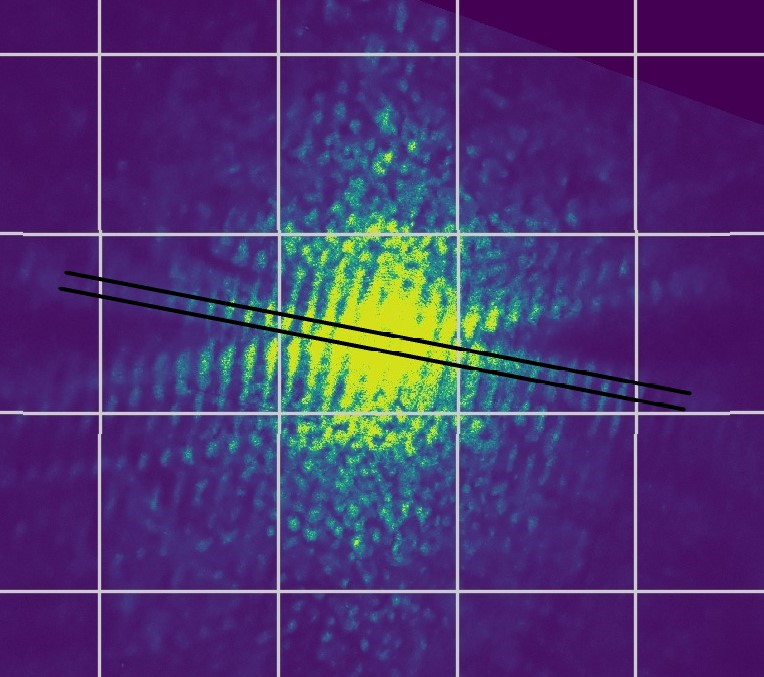
\includegraphics[width=\columnwidth]{figures/HelixSection3.jpg} % second figure itself
        \caption{"X" section 2}
        \label{fig:HelixSection4}
    \end{subfigure}
    \caption{Deconstruction of diffraction pattern to known 1D sections.}
    \label{fig:HelixSections}
\end{figure}

\subsection{Single slit section}
Taking the horizontal section of the helix we noticed that it can be described as:
\[T(x)\approx 1-rect\left(\frac{x}{2R}\right)\]
Where we treat the helix as approximately a cylinder, which is, in the context of our 1-D section (\ref{fig:HelixSection1}), the complement diffracting body of a single slit.
\begin{figure}[H]
    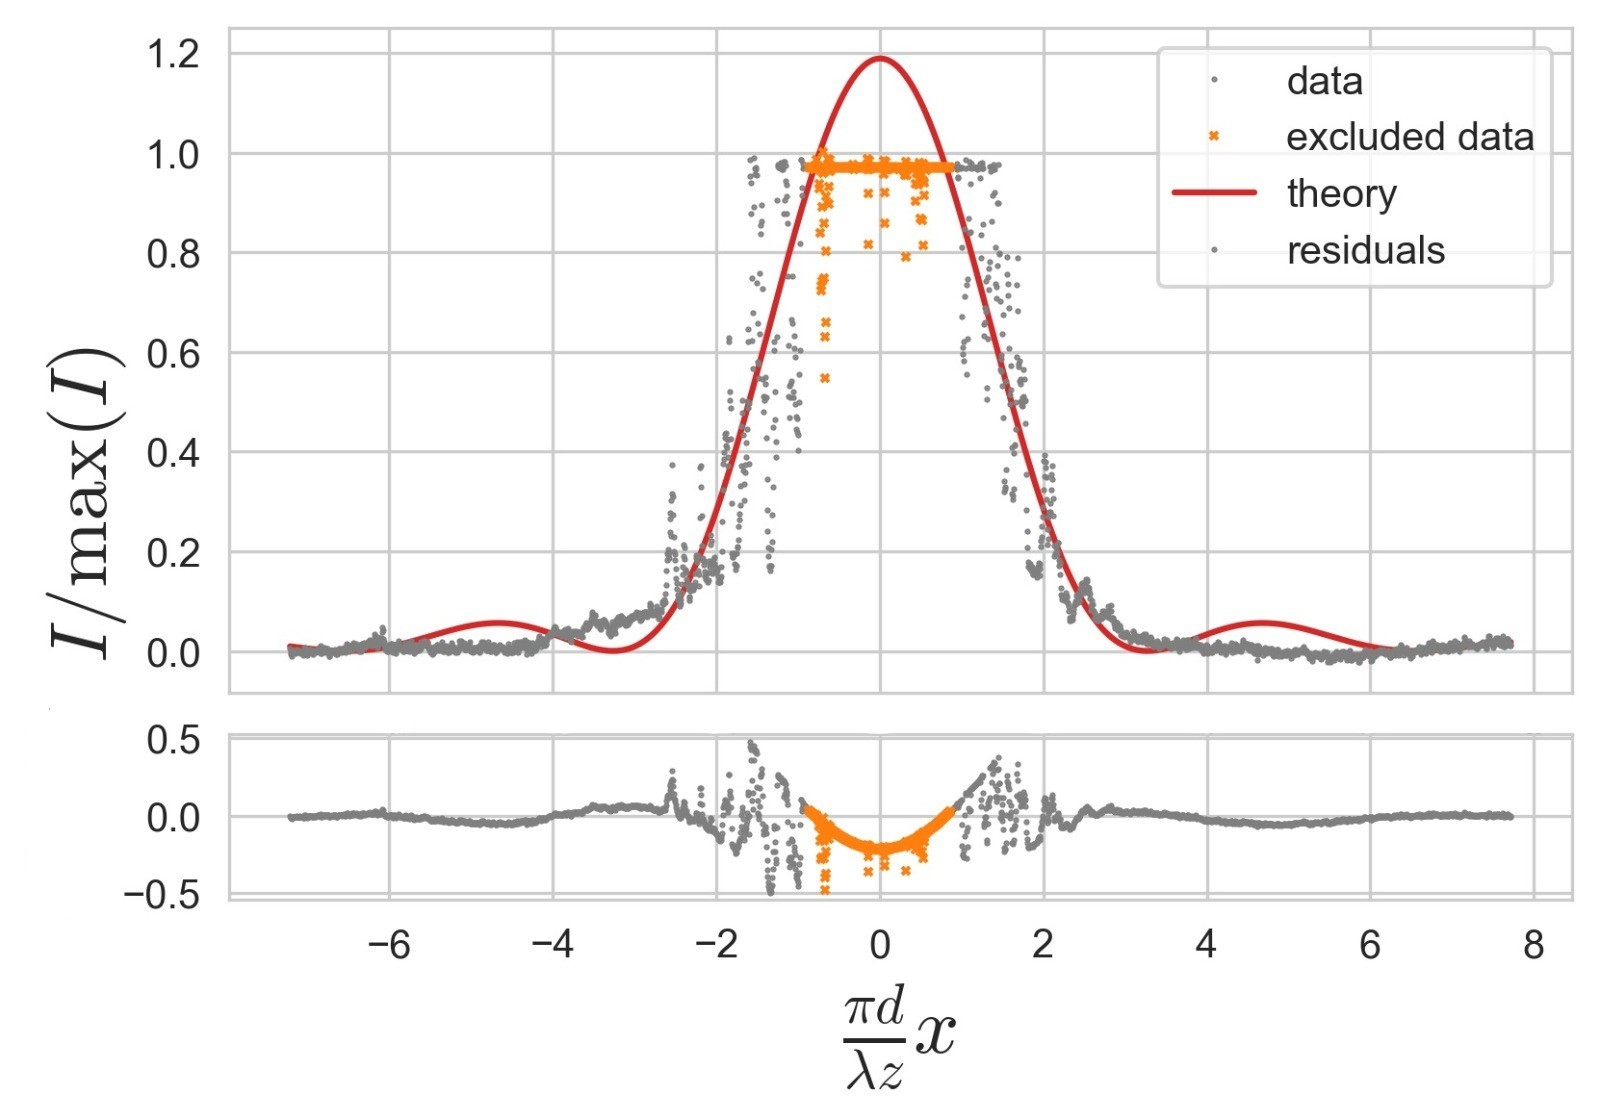
\includegraphics[width=0.9\columnwidth]{figures/Single slit section.jpeg}
    \caption{A fit for the single slit section of the helix using our model for single slit diffraction}
    \label{fig:Single slit section}
\end{figure}
The single slit model used in Figure~\ref{fig:Single slit section} describes the diffraction of our helix section with an error of $\sigma\approx0.1$.
The camera's sensor was saturated around $x=0$ and therefore that data was excluded from the fit.
We can also see oscillations around the main peak of the fit that increase in amplitude closer to $x=0$, we believe those are the result of the lack of focus in our picture.
There are oscillations in intensity along the "X" sections and the closer we get to the center of the single slit section the more they affect the intensity we measure.
\\
The radius of the helix according to the fit:
\[\]

\subsection{N slits section}
If we take the section perpendicular to that we've discussed earlier, there's a resemblance to the n slits pattern.
The width of the helix is now the distance between two slits, and the pitch is the width of each slit.
For the section taken along the middle of the helix we have: \[L=\frac{p}{2}-d',d'=\frac{d}{\sin \theta}\]
Where $d'$ is the width of the effective slit.
\begin{figure}[H]
    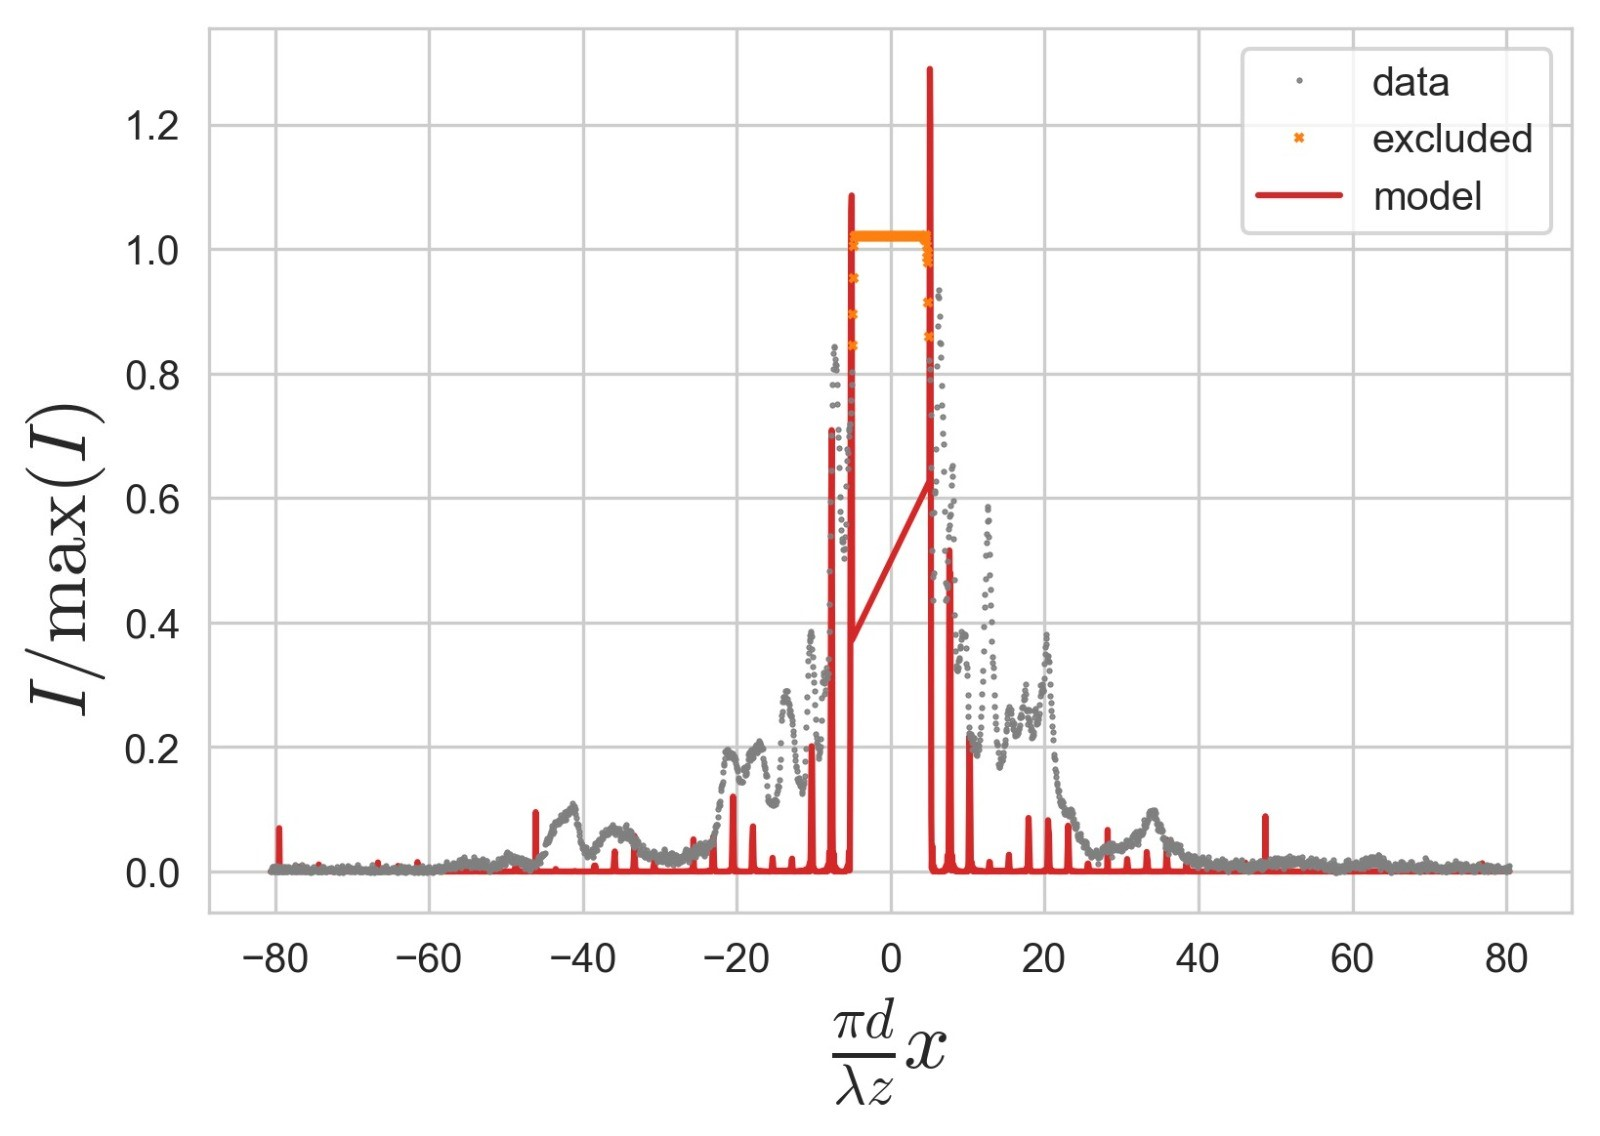
\includegraphics[width=0.9\columnwidth]{figures/n slits section.jpeg}
    \caption{A fit for the N-slits section using our model for N-slits diffraction}
    \label{fig:n slits section}
\end{figure}
Our model for N-slits is far from being able to predict the diffraction along the relevant section, we believe this is due to the focus problem discussed earlier.
While the model predicts some of the locations of local maxima, it fails to predict their amplitude and the behaviour of the pattern between those maxima.
The intensity changes faster relative to the single slit model and the focus effect is more dominant for this section.
We therefore decided not to rely on the parameters of the spring extrapolated from the fit.

\subsection{The "X" sections}
The two final sections are another way for us to compute the parameters of the slits.
In the example of N-slits section we saw that the locations of local maxima wasn't extremely affected by our measuring method.
We assume the same is true for the "X" sections (Fig.\ref{fig:X Sections}) and compute $d$ and $p$:
\[\]
Finally using some trigonometry we can get the following relation:
\[R=\frac{p}{4\tan \theta}+\frac{d}{2}\approx \]
The result is of the same scale as what we got from the fit for the single slit section.
